%\documentclass[landscape,a0b,final,a4resizeable]{a0poster}
%\documentclass[landscape,a0b,final]{a0poster}
%\documentclass[portrait,a0b,final,a4resizeable]{a0poster}
\documentclass[portrait,a0,final]{a0poster} %changed document class from a0b to a0 otherwise the second column extends out side the page

%%% Option "a4resizeable" makes it possible ot resize the
%   poster by the command: psresize -pa4 poster.ps poster-a4.ps
%   For final printing, please remove option "a4resizeable" !!

\usepackage{epsfig}
\usepackage{multicol}
\usepackage{pstricks,pst-grad}




%%%%%%%%%%%%%%%%%%%%%%%%%%%%%%%%%%%%%%%%%%%
% Definition of some variables and colors
%\renewcommand{\rho}{\varrho}
%\renewcommand{\phi}{\varphi}
\newrgbcolor{nus_blue}{0 0.129 0.388}
\newrgbcolor{nus_gold}{1 0.259 0}
\newrgbcolor{nus_lite}{1 0.259 0}
\newrgbcolor{lite}{.70 .70 .70}
\newrgbcolor{liter}{.95 .95 .95}
\setlength{\columnsep}{3cm}
% \setlength{\columnseprule}{2mm}
\setlength{\parindent}{0.0cm}


%% Figures and tables
%% The multicols package doesn't support the floats, figure and table.
%% Use tablehere and figurehere in place of table and figure.

\makeatletter
\newenvironment{tablehere}
  {\def\@captype{table}}
  {}

\newenvironment{figurehere}
  {\def\@captype{figure}}
  {}
\makeatother


% \figcaption replaces - replacement for \caption
% necessary, since in the multicols environment \figure and
% therefore \caption won't work

\newcommand{\ket}[1]{|{#1}\rangle}
\newcommand{\bra}[1]{\langle{#1}|}
\newcommand{\braket}[1]{\langle{#1}\rangle}

\setcounter{figure}{1}
\newcommand{\figcaption}[1]{
  \vspace{0.5cm}
  \begin{center}
  \begin{quote}
    {\large {\sc Figure} \arabic{figure}: #1}
  \end{quote}
  \end{center}
 % \vspace{1cm}
  \stepcounter{figure}
}

\setcounter{table}{1}
\newcommand{\tabcaption}[1]{
  \vspace{0.5cm}
  \begin{center}
  \begin{quote}
    {\normalsize {\sc Table} \arabic{table}: #1}
  \end{quote}
  \end{center}
 % \vspace{1cm}
  \stepcounter{table}
}
%%%%%%%%%%%%%%%%%%%%%%%%%%%%%%%%%%%%%%%%%%%%%%%%%%%%
%%%                Poster                        %%%
%%%%%%%%%%%%%%%%%%%%%%%%%%%%%%%%%%%%%%%%%%%%%%%%%%%%

\newenvironment{poster}{
  \begin{center}
  \begin{minipage}[c]{0.98\textwidth}
}{
  \end{minipage} 
  \end{center}
}




%%%%%%%%%%%%%%%%%%%%%%%%%%%%%%%%%%%%%%%%%%%%%%%%%%%%%%%%%%%%%%%%%%%%%%
%%% Begin of Document
%%%%%%%%%%%%%%%%%%%%%%%%%%%%%%%%%%%%%%%%%%%%%%%%%%%%%%%%%%%%%%%%%%%%%%

\begin{document}

\newrgbcolor{lightblue}{0. 0. 0.80}
\newrgbcolor{white}{1. 1. 1.}
\newrgbcolor{whiteblue}{.80 .80 1.}

\begin{poster}
\large \sf
\vspace{2cm}
%%%%%%%%%%%%%%%%%%%%%
%%% Header
%%%%%%%%%%%%%%%%%%%%%
\begin{center}

      %%% CQT_Logo
      \begin{minipage}[c]{0.05\textwidth}
        \begin{center}
          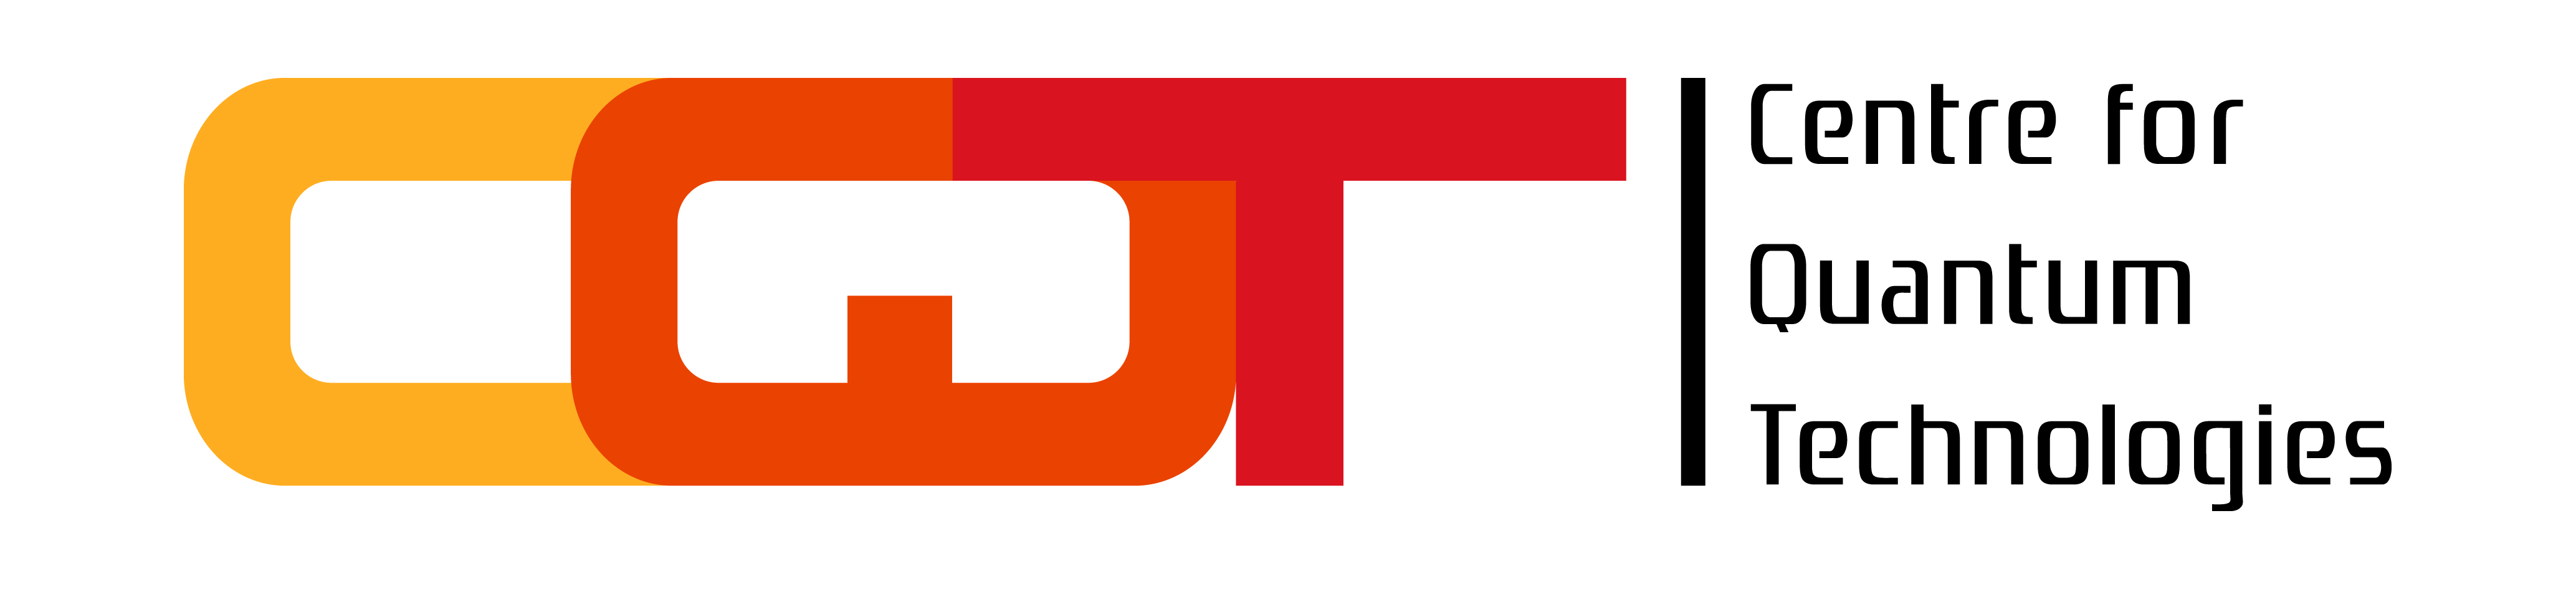
\includegraphics[width=14cm,angle=0]{CQT_Logo_CMYK.jpg}
        \end{center}
      \end{minipage}\hspace{10cm}
      %%% Title
      \begin{minipage}[c]{0.7\textwidth}
        \begin{center}
          {\sc \huge Strong Atom-Light Interaction in a Near-Concentric \\ \vspace{0.8cm}
          
Optical Resonator}\\[9mm]
          {\large Chi Huan Nguyen, Kadir Durak, Nick Lewty, Christian Kurtsiefer}\\[9mm]
          Centre for Quantum Technologies, National University of Singapore, Singapore\\
          
        \end{center}
      \end{minipage}
      %%% NUS-Logo
      \begin{minipage}[l]{0.1\textwidth}
        \begin{center}
          
\includegraphics[width=8cm,angle=0]{NUS_logo_full-horizontal.jpg}
        \end{center}
      \end{minipage}
\end{center}

\vspace{0.2cm}



%%%%%%%%%%%%%%%%%%%%%
%%% Content
%%%%%%%%%%%%%%%%%%%%%
\vspace{5cm}
\begin{multicols}{2}
\setlength{\parskip}{1ex plus 0.5ex minus 0.2ex}

      \begin{center}
          \begin{center}{\bf \Large \textsf {Motivation}}\end{center}
      \end{center}

 Strong interaction between an atom and a single photon can be successfully achieved by small mode volume cavities. Typically one would use short cavity lengths to achieve a small mode volume, but high finesse coatings are needed to ensure cavity losses remain less than the coupling strength. An alternative to this is to use a nearly concentric cavity, which achieves small mode volumes but with less stringent requirements on the dielectric coatings of the mirrors [1,2].

\begin{figurehere}

    \begin{multicols}{2}
        \begin{center}
            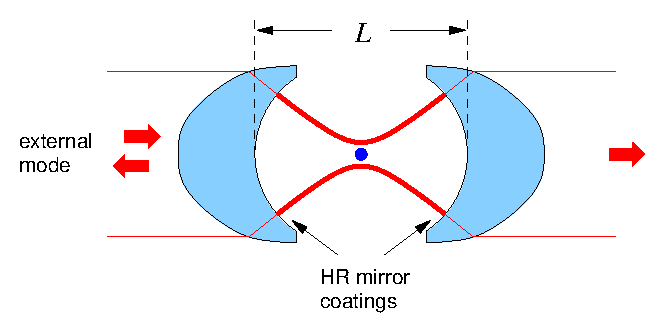
\includegraphics[width=\columnwidth]{cavitything}
            {
              
                $\qquad \mathrm{g_0}= \mathrm{E_f}\mathrm{d_{eff}} =
                \sqrt{\frac{\pi c R_{\mathrm{sc}}}{\tau L}}
            $}
    \columnbreak
    \hspace*{2cm}

            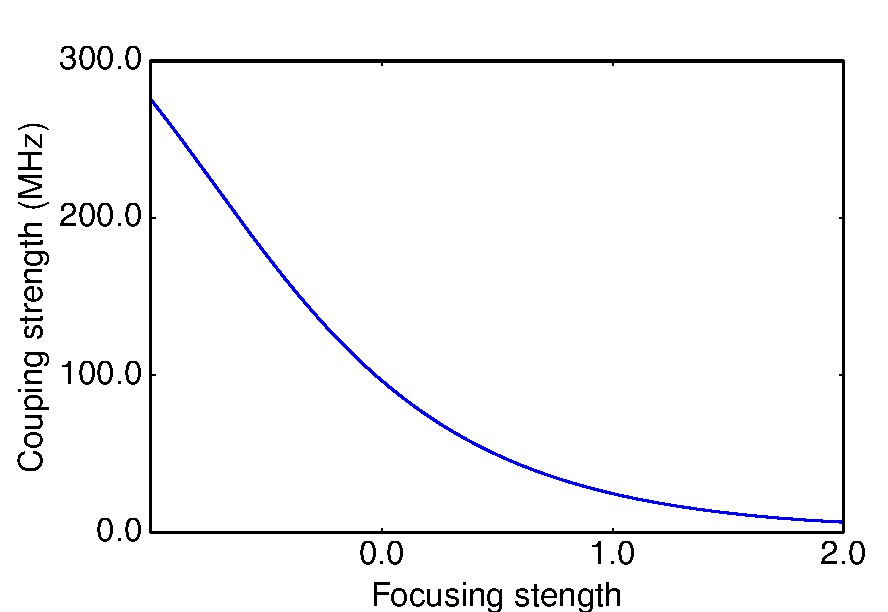
\includegraphics[width=\columnwidth]{coupling_strength.pdf}

        \end{center}
    \end{multicols}

  \figcaption{(Left) A nearly concentric optical cavity with a strongly focused mode. (Right) Coupling strength of the strongly focused mode on a closed transition of the $D_2$ line of $^{87}$Rb [2,3]. The focusing strength is the ratio of the input mode waist to half the cavity length.}

\end{figurehere}

\begin{center}
  {\bf \Large \textsf {Plano-convex cavity}}
\end{center}

Initially a cavity was setup with off the shelf plano-convex mirrors in order to understand the behaviour of a cavity in the near concentric regime.  Cavity linewidth and transmission measurements are made for different input beam waist sizes. The measurements are also simulated for comparison.


\begin{figurehere}
  \begin{center}
    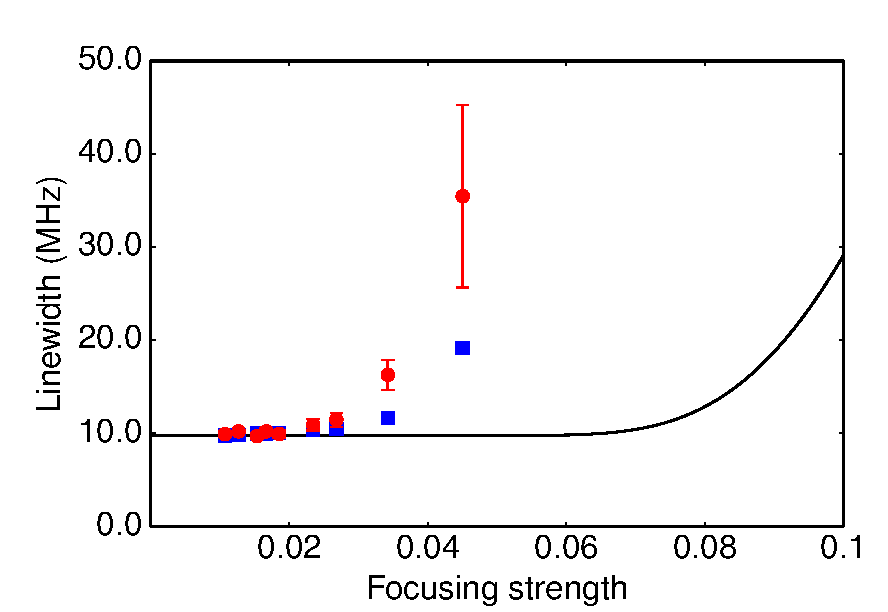
\includegraphics[width=0.7\columnwidth]{plano_convex_abberations.pdf}
    
  \end{center}
\end{figurehere}


\figcaption{The measured linewidth with plano-concave mirrors versus the focusing strength (red points). The black line corresponds to the model, taking only the diffraction loss into account. The blue points are the results of the simulation that consider both aberration and diffraction losses.}


The experimental results have some agreement with the simulated results on the effect of aberration on the cavity linewidth. Aberrations excite higher order modes, which can not be resolved as the mode separation is very close to the multiples of one free spectral range in the near concentric regime.



\begin{center}
     \begin{center} {\bf \Large \textsf {Anaclastic cavity}}\end{center}
\end{center}

An anaclastic design would reduce these aberrations in the input mode, which would reduce cavity losses below the cavity coupling rate, in the near concentric regime.

\begin{figurehere}
  \begin{center}
    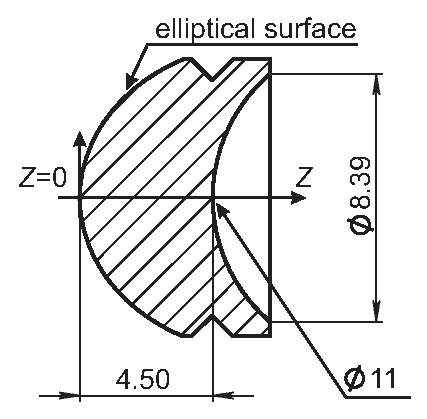
\includegraphics[width=0.3\columnwidth]{cavity_design}
   \hspace*{0cm}
    \includegraphics[width=0.5\columnwidth]{setup_sideon.png}
  \end{center}

  \figcaption{(Left) Anaclastic cavity mirror design. (Right) Anaclastic mirrors are controlled by a 3-axis PZTs for fine alignment.}
\end{figurehere}

\columnbreak

\begin{center}
     \begin{center} {\bf \Large \textsf {Anaclastic cavity characterisation}}\end{center}
\end{center}

Optical characterization of the anaclastic design show that the aberrative losses are reduced and higher order modes of the cavity are suppressed.

\begin{figurehere}
  \begin{center}
    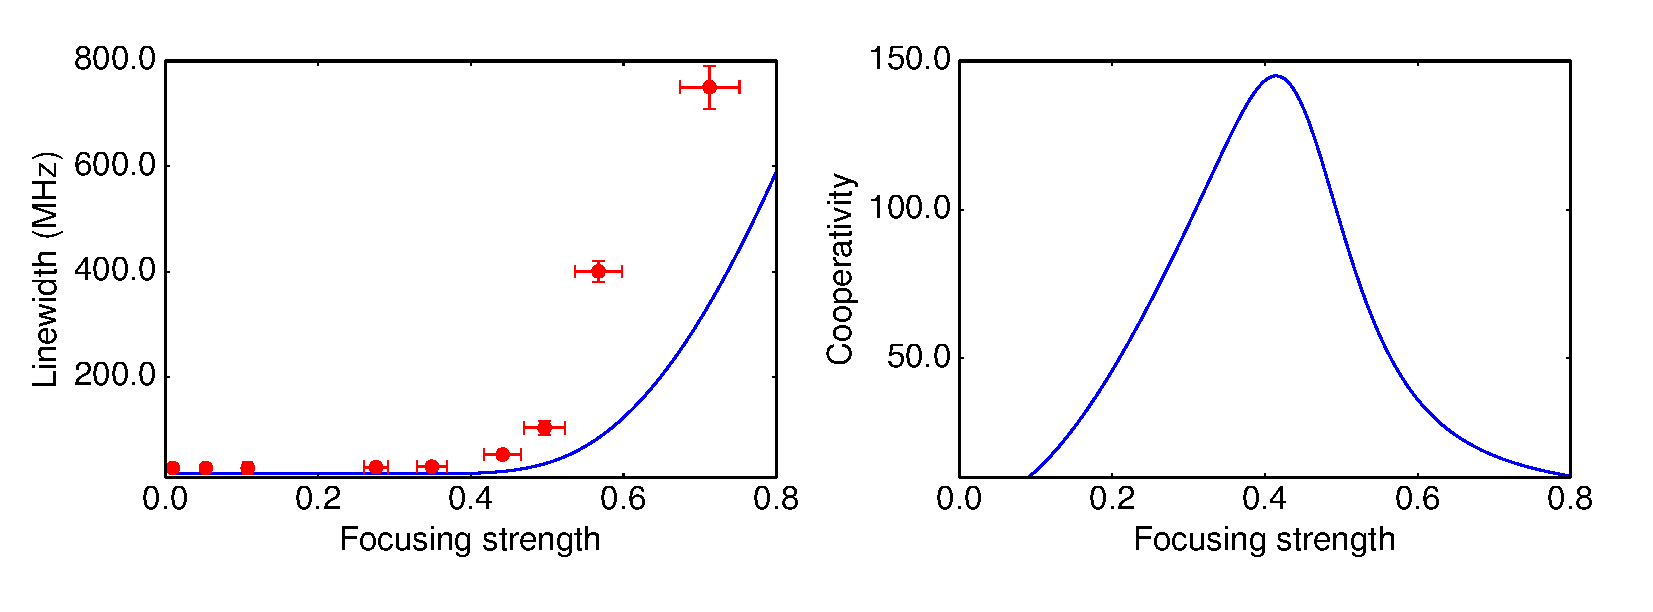
\includegraphics[width=\columnwidth]{plano_convex_abberations+cooperativity.pdf}
  \end{center}

\figcaption{(Left) Observed cavity linewidth versus the focusing strength. As the cavity becomes closer to the concentric limit, the finesse drops due to diffraction losses. The blue curve is a simulation of the linewidth which is limited only by diffraction losses. (Right) Estimated single atom cooperativity as a function of the focusing strength for the cavity coupled to the $D_2$ line of $^{87}$Rb. The single atom cooperativity peaks at a focusing strength of 0.4 due to the increase of the cavity linewidth caused by diffraction losses.}
\end{figurehere}


\begin{figurehere}
  \begin{center}
    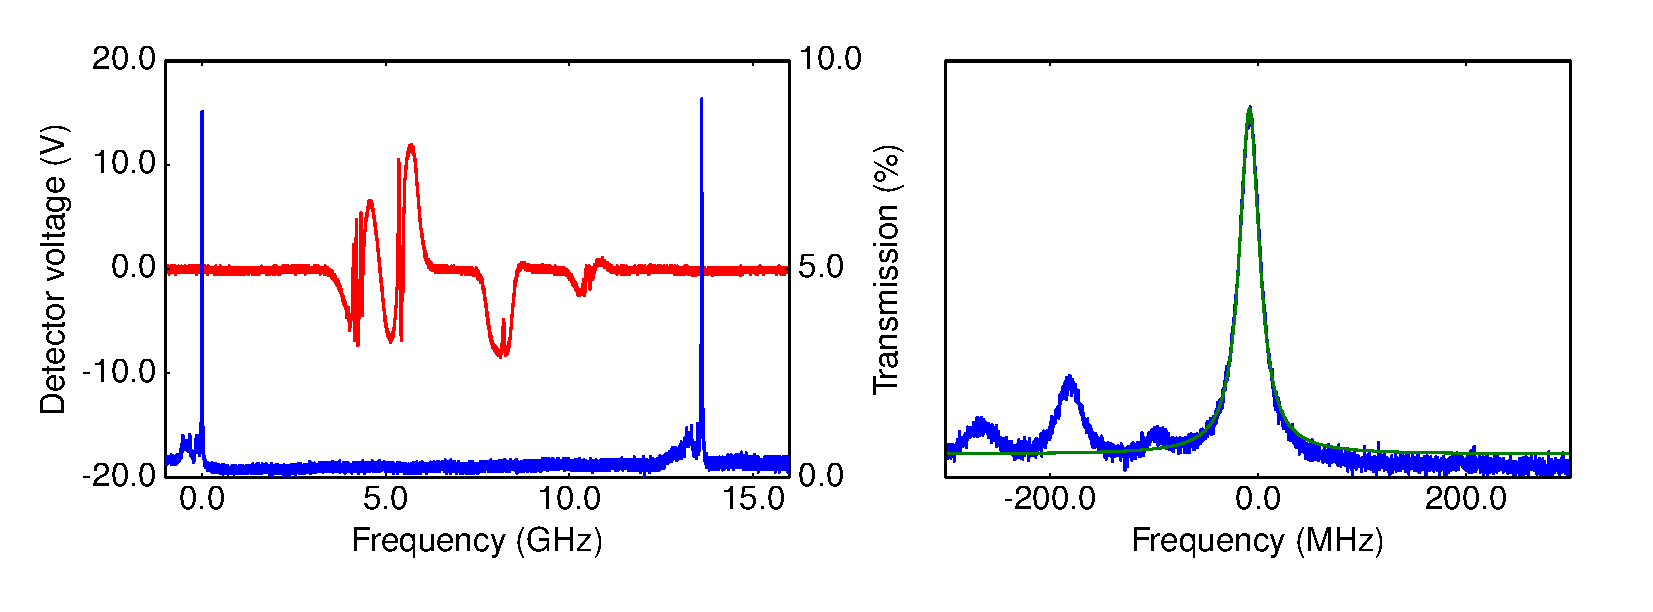
\includegraphics[width=\columnwidth]{cavity_fsr.pdf}
  \end{center}

\figcaption{(Left) The blue line shows the cavity transmission spectrum for a cavity which is 2.4$~\mu{m}$ shorter than the concentric cavity stability limit. The red line is an error signal from the hyperfine structure of the D$_2$ of $^{87}$Rb, which is shown as a frequency reference. (Right) Zoomed in cavity transmission showing fundamental mode and higher order modes, where the green line is the a fit of the fundamental mode.}
\end{figurehere}



\begin{center}
  {\bf \Large \textsf {Cavity enhanced collection of photons}}
\end{center}

We formed a MOT at the centre of the cavity mode and measured the number of photons leaking out of the cavity with an SPCM. The peaks in figure 6 are much larger than what would be expected from scattering, indicating an interaction between the cavity field and atoms from the MOT.

\begin{figurehere}
  \begin{center}
    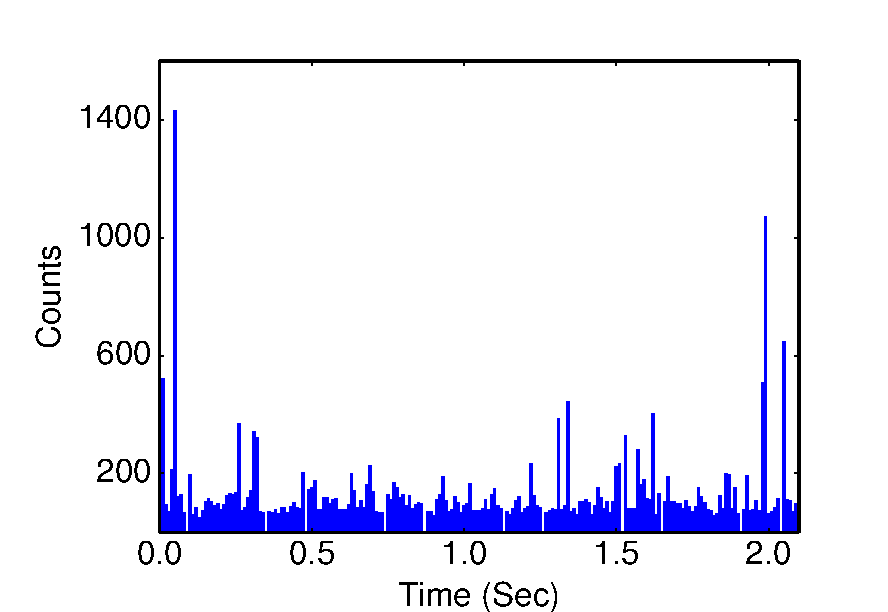
\includegraphics[width=0.7\columnwidth]{cavity_output_hist.pdf}
  \end{center}
    \figcaption{Histogram showing number of photons counted by a SPCM in 100$\,ms$ period. The data was generated by forming a MOT in the cavity mode and collecting the photons emitted from the cavity. The peaks represent a number of thermal atoms interacting with cavity mode. The cavity was left passively stable while performing the measurement.}
\end{figurehere}

\begin{flushleft}
       \begin{center}{\bf \large \textsf {References}}\end{center}
       [1] M.K. Tey et.al., New Journal of Physics {\textbf{11}}, 040311 (2009).
	\newline
         [2] S.E. Morin, et al., Phys.Rev.Lett., {\textbf {73}} pp.1411 (1994).
        \newline
	 [3] S.A. Aljunid et.al., Journal of Modern Optics, {\textbf{58}}, 299-305 (2011).

\end{flushleft}
    
\end{multicols}

\end{poster}

\end{document}

